\section{Biopython \& Scipy} \label{sec:MAFFT}

The colored trees were created by ETE3 with a newick file created with $N_{\text{PCA}}$ and $L_{\text{PCA}}$ and otherwise $N_{\text{UMAP}}$ and $L_{\text{UMAP}}$ (\autoref{fig:PCA_Clusteree_Knee_4}, \autoref{fig:UMAP_Clusteree_Knee_4}) \autocite{huerta-cepas_ete_2016}. The newick file was created with a feature request proposed for the \textbf{scipy} package version 1.6.0 involving the \textbf{cluster.hierarchy.to\_tree} function as described in the \href{https://github.com/scipy/scipy/issues/8274}{issue}\footnote{last accessed 02/06/21} (\autoref{fig:Tree_Pipeline} \textsf{\textbf{J}}) \autocite{scipy_10_contributors_scipy_2020}.

\begin{leftbar}
    %\textbf{mafft}
    \textbf{scipy.cluster.hierarchy.to\_tree}
    \begin{nstabbing}
        \qquad\qquad\qquad\qquad\qquad\quad\=\kill
    
        Z \> [input linkage matrix]
    \end{nstabbing}
\end{leftbar}

For chosing all the clusters centroid sequences $C$ which are a subset of all the genomic sequences $S$, the \textbf{spatial.distance.cdist} function also from the \textbf{scipy} package was used (\autoref{fig:Tree_Pipeline} \textsf{\textbf{K}}) \autocite{scipy_10_contributors_scipy_2020}. Let $S_{N=o}$ be the subset of $S$ matching the cluster $o$ in $N$ and $\mathbf{\hat{X}}_{N=o}$ the normalized matrix of $S_{N=o}$. The centroid sequence $C_o$ of the cluster $o$ is the sequence $S_i$ of $S_{N=o}$ where sum of the cosine distance of vector representation $\mathbf{\hat{x}}_i$ to all the other $k$ vectors of $\mathbf{\hat{X}}_{N=o}$ is equal the minimum of the \textbf{spatial.distance.cdist} function with the normalized matrix $\mathbf{\hat{X}}_{N=o}$ of $S_{N=o}$ and \colorbox{backcolour}{metric='cosine'} \autoref{eq:centroid}.

\begin{empheq}{alignat = -1}
    &\min \left( \text{CDIST}_{\text{cos}}(\mathbf{\hat{X}}_{N=o}, \mathbf{\hat{X}}_{N=o}) \right) &&= \sum^k_{j=1} d_{\text{cos}}(\mathbf{\hat{x}}_i, \mathbf{\hat{x}}_j ) \Rightarrow C_o = S_i\label{eq:centroid}
\end{empheq}

The materials named in the following are only used for the analyses in the \autoref{sec:Clustering_Anomalies} to \autoref{sec:Dimension_Reduction} and therefore not part of the proposed raw clustering tool (\autoref{fig:Alignment_Pipeline} and \autoref{fig:Precalc_Pipeline}).

\begin{figure}[!hbt]
    \centering
    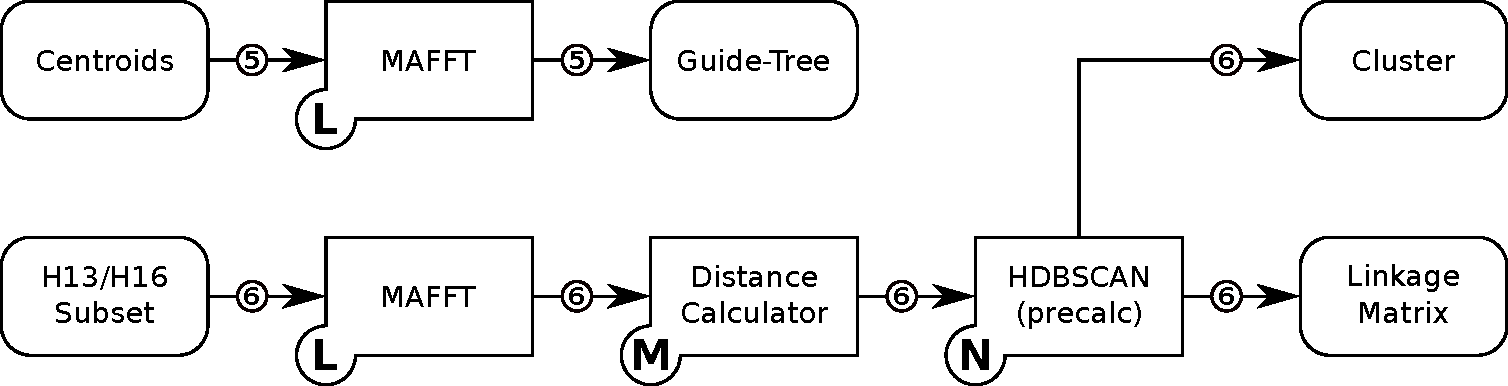
\includegraphics[width=\textwidth]{Graphics/Alignment.pdf}
    \caption[Alignment Pipeline]{\textbf{Alignment Pipeline.} }
    \label{fig:Alignment_Pipeline}
\end{figure}

\begin{figure}[!hbt]
    \centering
    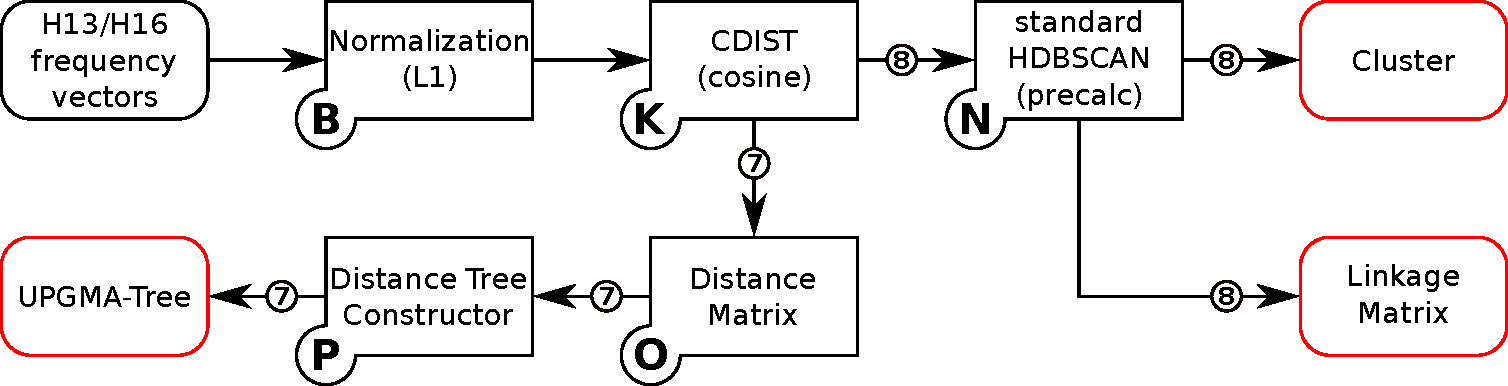
\includegraphics[width=\textwidth]{Graphics/Precalculated.pdf}
    \caption[Precalculation Pipeline]{\textbf{precalculation Pipeline.} }
    \label{fig:Precalc_Pipeline}
\end{figure}

The Biopython implementation of MAFFT version 7.475 from the \textbf{biopython (Bio)} package version 1.78 was used to build the guidetrees in \autoref{sec:Clustering_Anomalies} according to \autoref{fig:Alignment_Pipeline} pathway \textsf{\textbf{5}} with the genomic sequences of the centroids $C$ \autocite{katoh_mafft_2013, cock_biopython_2009} (\autoref{fig:Alignment_Pipeline}. The settings were mostly the default settings proposed in the \href{https://mafft.cbrc.jp/alignment/software/}{manual}. For faster execution \colorbox{backcolour}{thread=6} and for export of the guidetree \colorbox{backcolour}{treeout=True} setting was used \autocite{katoh_mafft_2013, cock_biopython_2009}. The guide-tree was colored with ETE3 (\autoref{fig:Alignment_Pipeline} \textsf{\textbf{K}}) \autocite{huerta-cepas_ete_2016}.

The parameters used in this project with settings varying from the default are listed below. All available settings can be fount in the \href{https://mafft.cbrc.jp/alignment/software/}{manual}.

\begin{leftbar}
    %\textbf{mafft}
    \textbf{Bio.Align.Applications.MafftCommandline}
    \begin{nstabbing}
        \qquad\qquad\qquad\qquad\qquad\quad\=\kill
    
        treeout \> [export guidetree used for alignment (default: off)]\\
        
        thread \> [number of used threads (default: 1)]\\
        
        input \> [input FASTA file]
        
        %-{}-{}6merpair \> (default: on)\\
        %\> input\\
        %> \> output
    \end{nstabbing}
\end{leftbar}

In \autoref{sec:Comparison_Clustering} five different cluster trees are compared to each other. The trees are based on clustering with \gls{HDBSCAN}, without hybrid clustering ($\varepsilon=0$) \autocite{malzer_hybrid_2020, mcinnes_hdbscan_2017}. For each clustering a different matrix was used as input. The trees of \gls{UMAP} and \gls{PCA} (\autoref{fig:Simple_Clustertree_PCA} and \autoref{fig:Simple_Clustertree_UMAP}) were created according to \autoref{fig:Vectorization_Pipeline} and \autoref{fig:Clustering_Pipeline} and as described in \autoref{sec:Frequency} to \autoref{sec:HDBSCAN} with a smaller FASTA subset $S_{\text{Sub}}$, consisting only of $o$ segment 4 sequences with subtypes H13 and H16 and a resulting smaller matrix $\mathbf{\hat{X}}_{\text{Sub}}$. Therefore clustering for the trees of \gls{UMAP} and \gls{PCA} were executed with matrix $\mathbf{\hat{X}}_{\text{Sub, (30)}}$ and $\mathbf{Y}_{\text{Sub}}$. Sub denotes the matrix variant with smaller subset (\autoref{eq:hdb_prime_x} and \autoref{eq:hdb_prime_y}). 

\begin{empheq}{alignat = -1}
    &N_{\text{PCA, Sub}} &&= \text{HDBSCAN} (\mathbf{\hat{X}}_{\text{Sub, (30)}}, 2, 1, 0)\label{eq:hdb_prime_x}\\
    &N_{\text{UMAP, Sub}} &&= \text{HDBSCAN} (\mathbf{Y}_{\text{Sub}}, 2, 1, 0)\label{eq:hdb_prime_y}
\end{empheq}

The two trees based the clustering with precalculation (\autoref{fig:Simple_Clustertree_Cosine} and \autoref{fig:Simple_Clustertree_Euclid}) were created by distance calculation on the $\mathbf{X}_{\text{Sub}}$ matrix. For the calculation of the distance the \textbf{scipy} package version 1.6.0 was used with the \textbf{spatial.distance.cdist} function (\autoref{fig:Precalc_Pipeline} \textsf{\textbf{N}}) \autocite{scipy_10_contributors_scipy_2020}. For calculation of the cosine distance \colorbox{backcolour}{matric='cosine'} and for euclidean distance \colorbox{backcolour}{metric='euclidean'} setting was used (\autoref{eq:c_calc_matrix} to \autoref{eq:e_calc_matrix}). The resulting distance matrizes $\mathbf{C}_{\text{Sub}}$ and $\mathbf{E}_{\text{Sub}}$ were clustered with \gls{HDBSCAN} and \colorbox{backcolour}{metric='precalculated'} setting (\autoref{fig:Precalc_Pipeline} \textsf{\textbf{F}} and \autoref{eq:hdb_prime_e} to \autoref{eq:hdb_prime_c}) \autocite{mcinnes_hdbscan_2017}.

% \begin{empheq}{alignat = -1}
%     &c_{i,j} &&= d_{\text{cos}}(\mathbf{x}_i, \mathbf{x}_j), \ i = 1, \ldots o, \ j = 1, \ldots o\label{eq:c_calc_1}\\
%     &&&= 1 - \frac{\mathbf{x}_i^\top\mathbf{x}_j}{\Vert\mathbf{x}_i\Vert \cdot \Vert\mathbf{x}_j\Vert}\label{eq:c_calc_2}
% \end{empheq}

\begin{empheq}{alignat = -1}
    &\mathbf{C}_{\text{Sub}} &&= \text{CDIST}_{\text{cosine}}(\mathbf{X}_{\text{Sub}}, \mathbf{X}_{\text{Sub}}) \label{eq:c_calc_matrix}\\
    &\mathbf{E}_{\text{Sub}} &&= \text{CDIST}_{\text{euclidean}}(\mathbf{X}_{\text{Sub}}, \mathbf{X}_{\text{Sub}}) \label{eq:e_calc_matrix}
\end{empheq}

\begin{empheq}{alignat = -1}
    &N_{\text{eucl, Sub}} &&= \text{HDBSCAN} (\mathbf{E}_{\text{Sub}}, 2, 1, 0)\label{eq:hdb_prime_e}\\
    &N_{\text{cos, Sub}} &&= \text{HDBSCAN} (\mathbf{C}_{\text{Sub}}, 2, 1, 0)\label{eq:hdb_prime_c}
\end{empheq}

\begin{leftbar}
    \textbf{scipy.spatial.distance.cdist}
    \begin{nstabbing}
        \qquad\qquad\qquad\qquad\qquad\quad\=\kill
    
        metric \> [Distance metric for calculation (default: 'euclidean')]

    \end{nstabbing}
\end{leftbar}

The last of the five trees is based on MAFFT with the \textbf{biopython} package. The alignment was done on the subset $S_{\text{Sub}}$. On the alignment the distance matrix was calculated by the \textbf{Phylo.TreeConstruction.DistanceCalculator} function from the \textbf{biopython (Bio)} package. The standard settings for nucleotide sequences was used for the calculation \colorbox{backcolour}{model='identity'} \autocite{cock_biopython_2009}.

\begin{empheq}{alignat = -1}
    &\mathbf{G}_{\text{Sub}} &&= \text{DistanceCalculator}_{\text{identity}}(\text{MAFFT}(S_{\text{Sub}}))
\end{empheq}

\begin{leftbar}
    \textbf{Bio.Phylo.TreeConstruction.DistanceCalculator}
    \begin{nstabbing}
        \qquad\qquad\qquad\qquad\qquad\quad\=\kill
    
        model \> [model for distance calculation (default: 'identity')]

    \end{nstabbing}
\end{leftbar}

The \textbf{Phylo.TreeConstruction.DistanceMatrix} and \textbf{DistanceTreeConstructor} function also from the \textbf{biopyhton} package was used for calculation of precalculated UPGMA trees in \autoref{sec:K_mer_Representation}. Instead of the default neighbor joining setting, the bottom-up hierarchical clustering method \colorbox{backcolour}{method='upgma'} was used (\autoref{fig:Alignment_Pipeline} \textsf{\textbf{P}} and \textsf{\textbf{P}}) \autocite{gower_minimum_1969, cock_biopython_2009}. The matrices calculated in \autoref{eq:c_calc_matrix} and \autoref{eq:e_calc_matrix} were used as input for the calculation of the UPGMA-trees \autocite{sokal_statistical_1958}.

\begin{leftbar}
    \textbf{Bio.Phylo.TreeConstruction.DistanceMatrix}
    \begin{nstabbing}
        \qquad\qquad\qquad\qquad\qquad\quad\=\kill
    
        names \> [name of columns and rows]\\
        
        matrix \> [input matrix]
    \end{nstabbing}
\end{leftbar}

\begin{leftbar}
    \textbf{Bio.Phylo.TreeConstruction.DistanceTreeConstructor}
    \begin{nstabbing}
        \qquad\qquad\qquad\qquad\qquad\quad\=\kill
    
        method \> [construction method for the distance tree (default: 'nj')]
        
    \end{nstabbing}
\end{leftbar}